\documentclass[a4paper,10pt]{IEEEtran}
\usepackage{mathptmx}

\usepackage{tabularx} % extra features for tabular environment
\usepackage{amsmath}  % improve math presentation
\usepackage{float}
% \usepackage{pdfpages}

\usepackage{subfig}

\usepackage{graphicx} % takes care of graphics including machinery
\graphicspath{ {./figures_final/} }
%\usepackage[margin=1in,letterpaper]{geometry} % decreases margins
%\usepackage{cite} % takes care of citations
\usepackage[final]{hyperref} % adds hyperlinks inside the generated pdf file
\hypersetup{
    colorlinks=true,       % false: boxed links; true: colored links
    linkcolor=blue,        % color of internal links
    citecolor=blue,        % color of links to bibliography
    filecolor=magenta,     % color of file links
    urlcolor =blue         
}
\usepackage[margin = 1in,headsep=0.5cm,headheight=2cm,letterpaper]{geometry} 

\usepackage{fancyhdr}
\pagestyle{fancy}
\lhead{Student 1 : Ahmet Akman 2442366 \\ Student 2: Kaan Demirkoparan 2442903}
\rhead{Date: \today \\ Group: Friday Morning - 6} 
%\cfoot{center of the footer!}
%\renewcommand{\headrulewidth}{0.1pt}

\title{  EE313 Fall 2022 Project Work  \protect\\ Final Report}
\author{ Ahmet Akman 2442366 -- Kaan Demirkoparan 2442903 }
\date{}
\begin{document}
\thispagestyle{empty}


\maketitle
%\tableofcontents
%\begin{abstract}
%abstract
%\end{abstract}

\section{Introduction}
Our project in the fall semester of 2022 aimed to transmit an audio signal via an optical transmitter module. It was divided into two components: the transmitter and receiver. To measure signal strength, we combined the audio signal with a reference signal. Our design featured circuit designs such as low-pass and high-pass filters, an automatic gain control circuit, and a power amplifier for the speaker. This report will give details on the project's specifications, components, and stages. It will also provide information on the design methodology, simulation results, experimental results, a comparison of the simulation and experimental results, and explanations for any differences.
\section{General Structure and Design Philisophy}
 The general structure is given in Figure \ref{general}
\begin{figure}[htbp!]
    \centering
    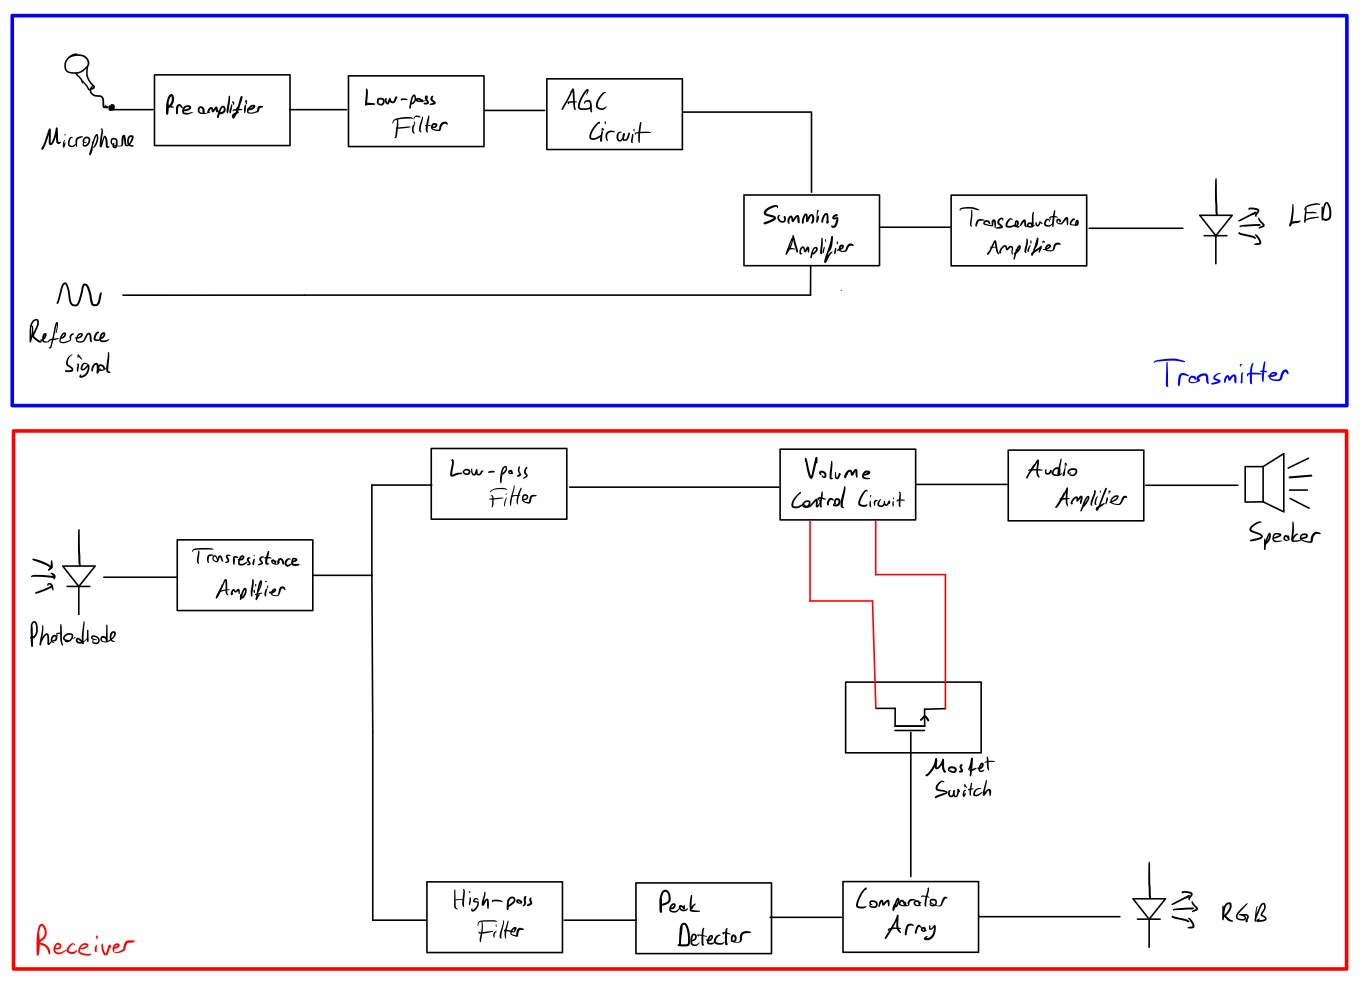
\includegraphics[width = 1\linewidth]{general_structure.jpeg}
    \caption{General Structure}
    \label{general}
\end{figure} 
\section{Transmitter Side}
\subsection{Input and Early Stage Amplification}
The microphone functions as a resistor, with its resistance varying based on the audio waves. To turn audio signals into electrical signals, a voltage divider circuit can be employed. However, the resulting output signal is quite weak, making it susceptible to noise. To mitigate this, the small signal is amplified using a common source or common emitter amplifier, which results in a less noise-sensitive and more usable voltage range signal. Subsequently, this signal is passed through a low pass filter to separate the human voice for further processing. The schematic of this circuit is given in Figure \ref{PreAmp}

\begin{figure}[htbp!]
    \centering
    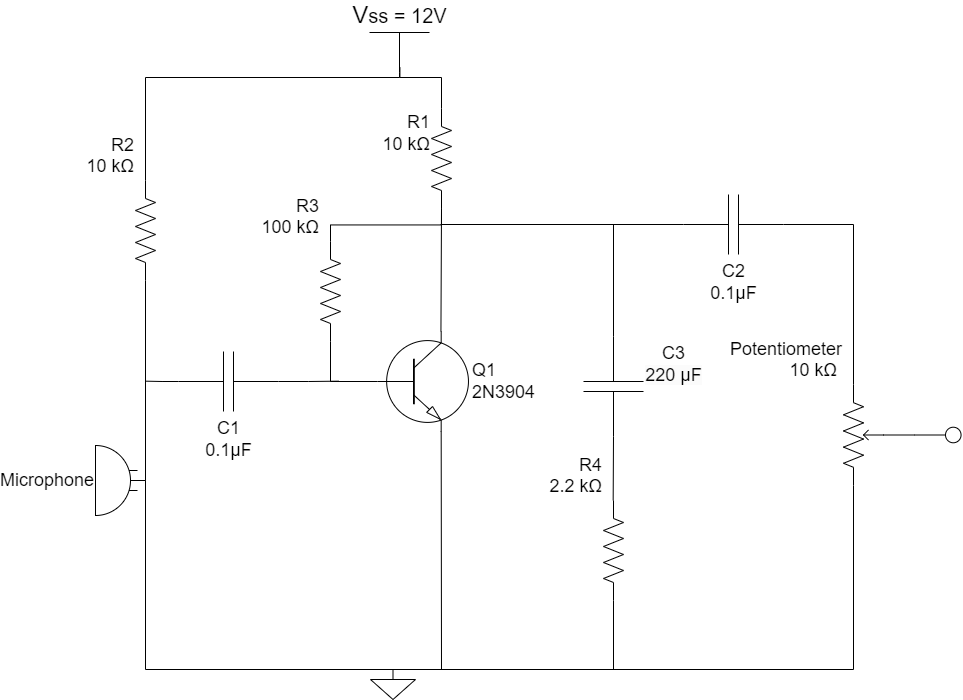
\includegraphics[width = 1\linewidth]{Preamplifier.drawio.png}
    \caption{Microphone and preamplification circuit}
    \label{PreAmp}
\end{figure} 
The amplification factor can be adjusted from the pot so that the voice level and noise level can be fine tuned with a proper selection of amplification factor. The construction of this circuit is done on a breadboard and it can be said that the design specs are satisfied successfully as shown in the demonstration. The experimental output of the preamplification is given in Figure \ref{preamp_osc}. The input is a 1khz sine wave sound played from a device.
\begin{figure}[htbp!]
    \centering
    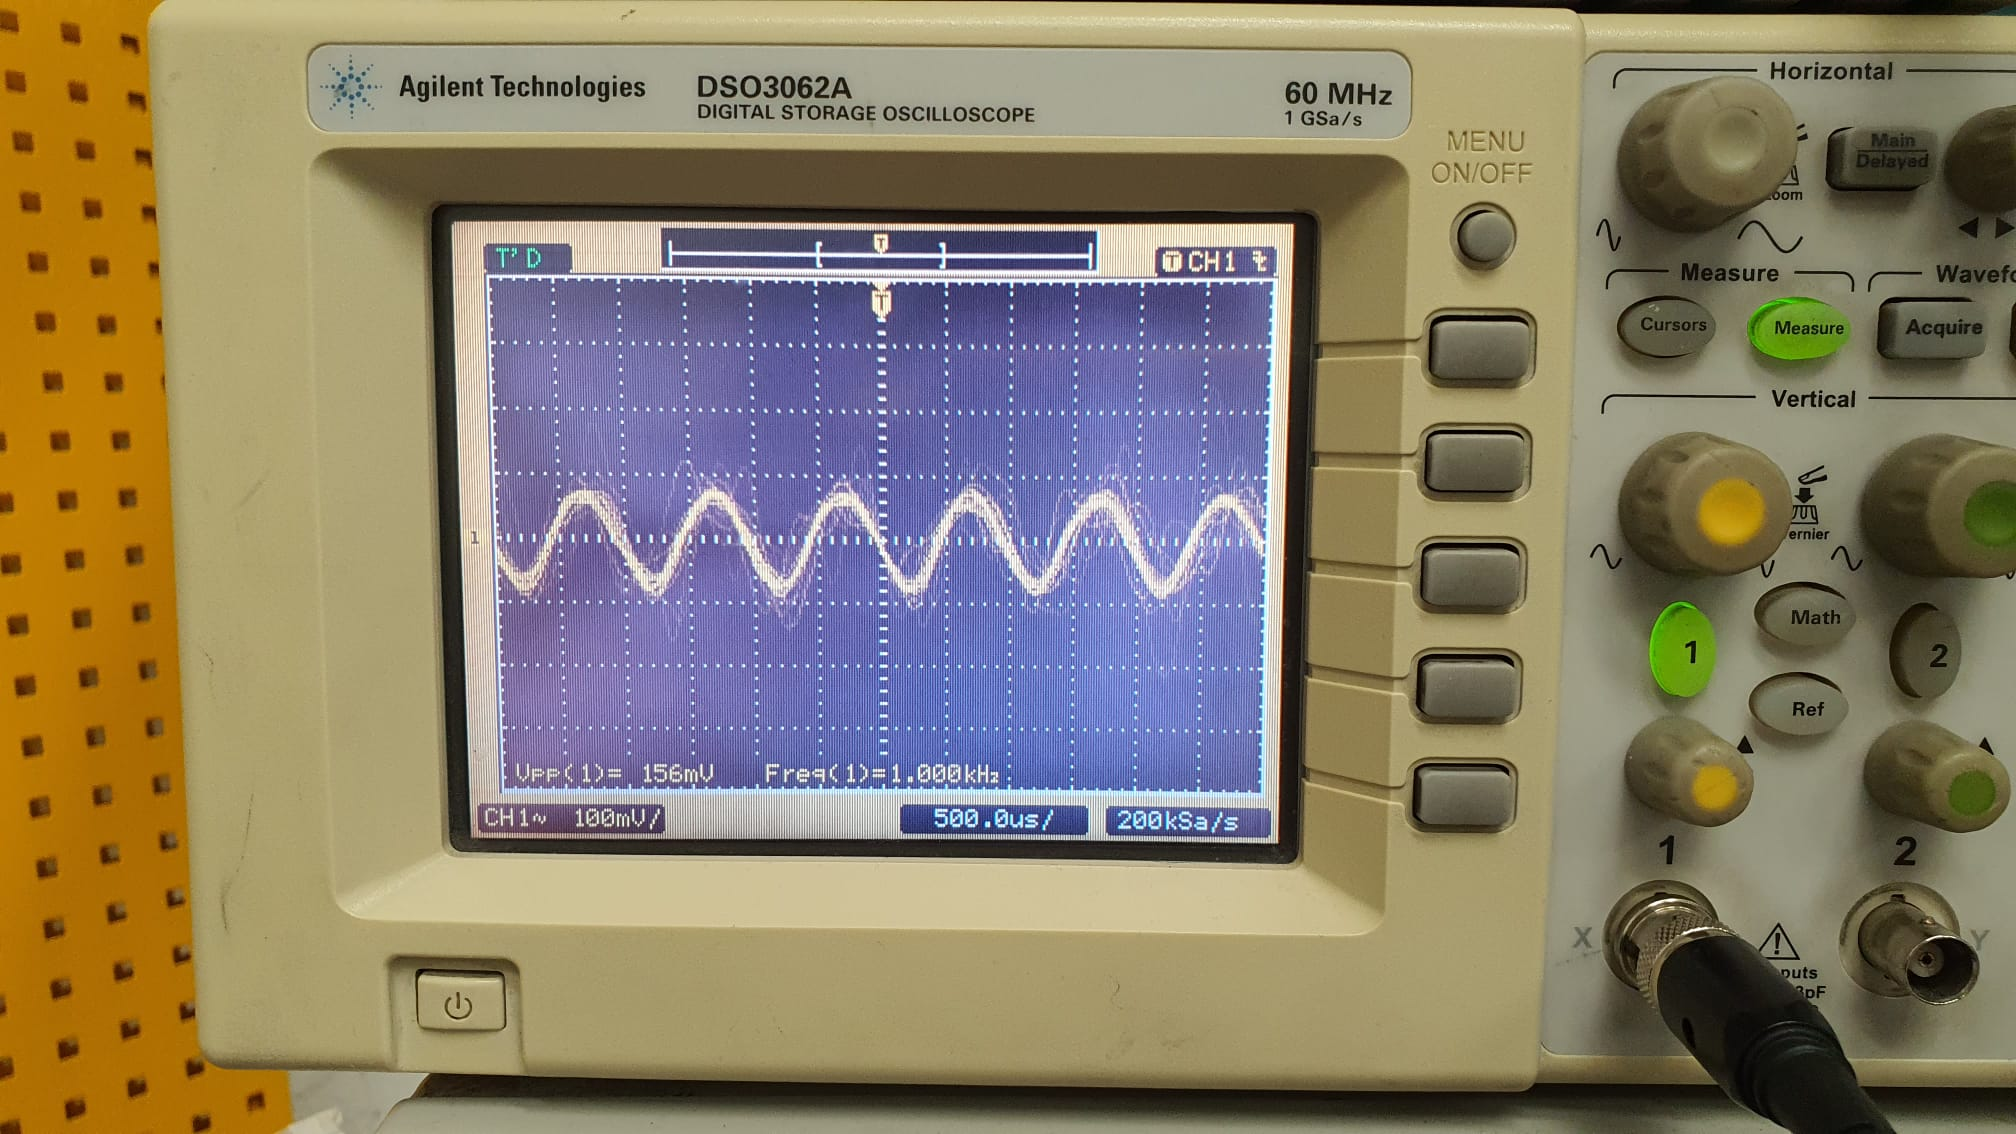
\includegraphics[width = 1\linewidth]{preamp_experimental.jpeg}
    \caption{Microphone and preamplification circuit experimental result.}
    \label{preamp_osc}
\end{figure} 


\subsection{Low Pass Filter}
After the preamplification process is completed, the resulting output signal is sent to a low-pass filter to remove any unwanted frequencies. The typical range of human hearing is between 20 Hz and 20 kHz, but for this specific project, only the range of 100 Hz to 5 kHz is used. This is done to prevent overlap between the audio signal and the reference signal in the frequency domain. The low-pass filter used in this project is a two stage sallen-key active low pass filter which is shown in Figure \ref{lowpass}
\begin{figure}[htbp!]
    \centering
    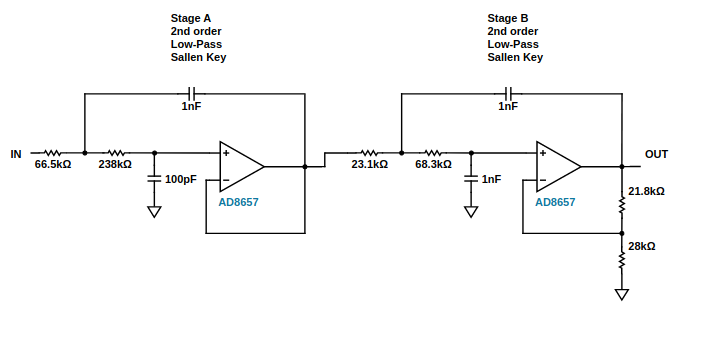
\includegraphics[width = 1\linewidth]{active_low_pass_circuit.png}
    \caption{Active low pass filter.}
    \label{lowpass}
\end{figure} 
The frequency response of the circuit is given in Figure \ref{lowpass_resp}.
\begin{figure}[htbp!]
    \centering
    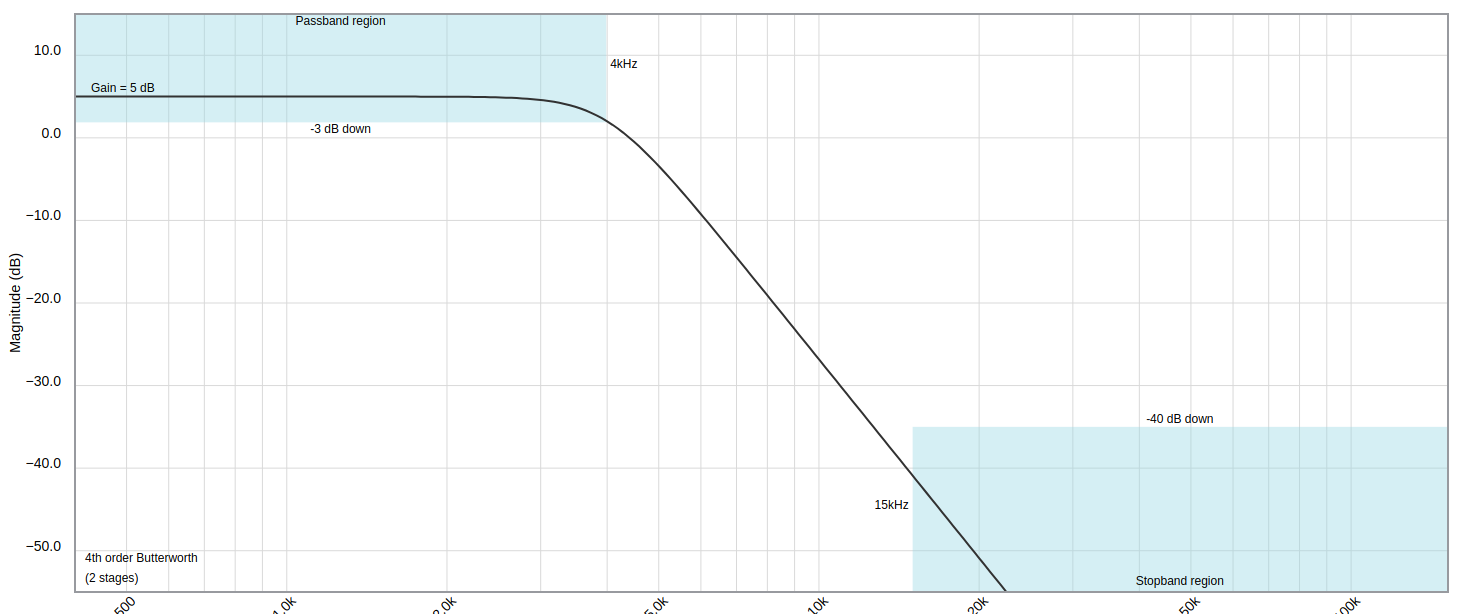
\includegraphics[width = 1\linewidth]{active_low_pass.png}
    \caption{Active low pass filter frequency response.}
    \label{lowpass_resp}
\end{figure} 
The filtering strategy is observed to be quite accurate decision as very small noise is measured from the output. 
\subsection{Automatic Gain Control}
The automatic gain control circuit given in Figure \ref{AGC} is designed.

\begin{figure}[htbp!]
    \centering
    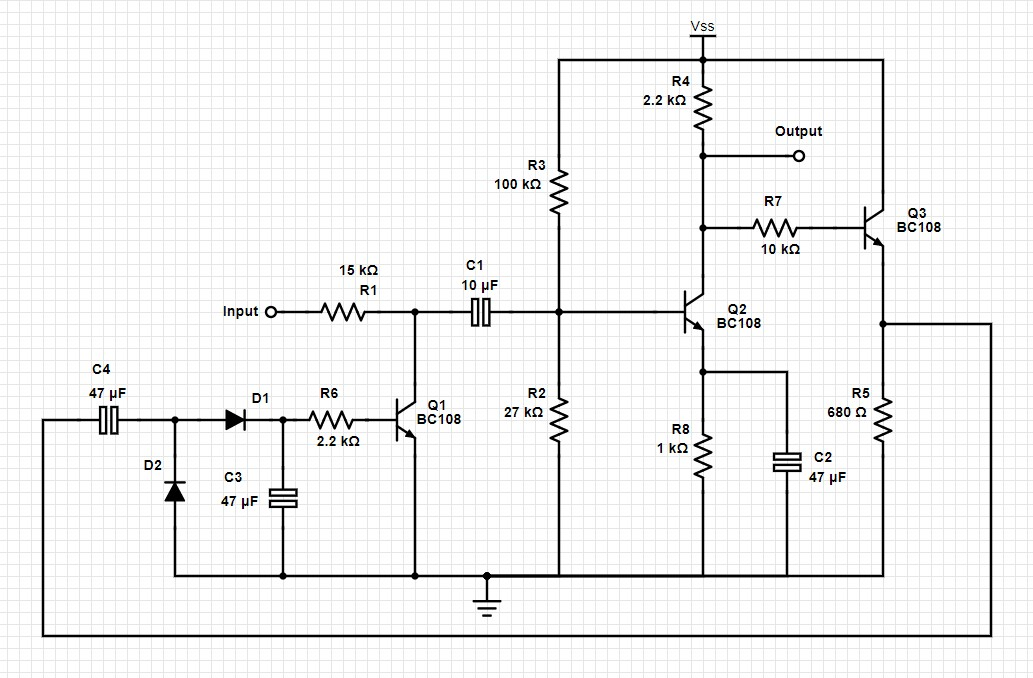
\includegraphics[width = 1\linewidth]{AGC Circuit.jpg}
    \caption{Automatic gain circuit schematic.}
    \label{AGC}
\end{figure} 
 The circuit composed of three transistors. The first stage (Q2) is a common emitter amplifier with a feedback supplied by other two transistor. The second transistor in common collector configuration is a voltage buffer that takes the amplitude information of the Q2. Then the Q3 works as an active resistor which takes input from a simple peak detector connected after Q3. 
 The simulation carried out in LTSpice .The  input and output characteristics for different amplitudes are given in Figure \ref{AGC_sim_input} and \ref{AGC_sim_output} respectively.
 \begin{figure}[htbp!]
    \centering
    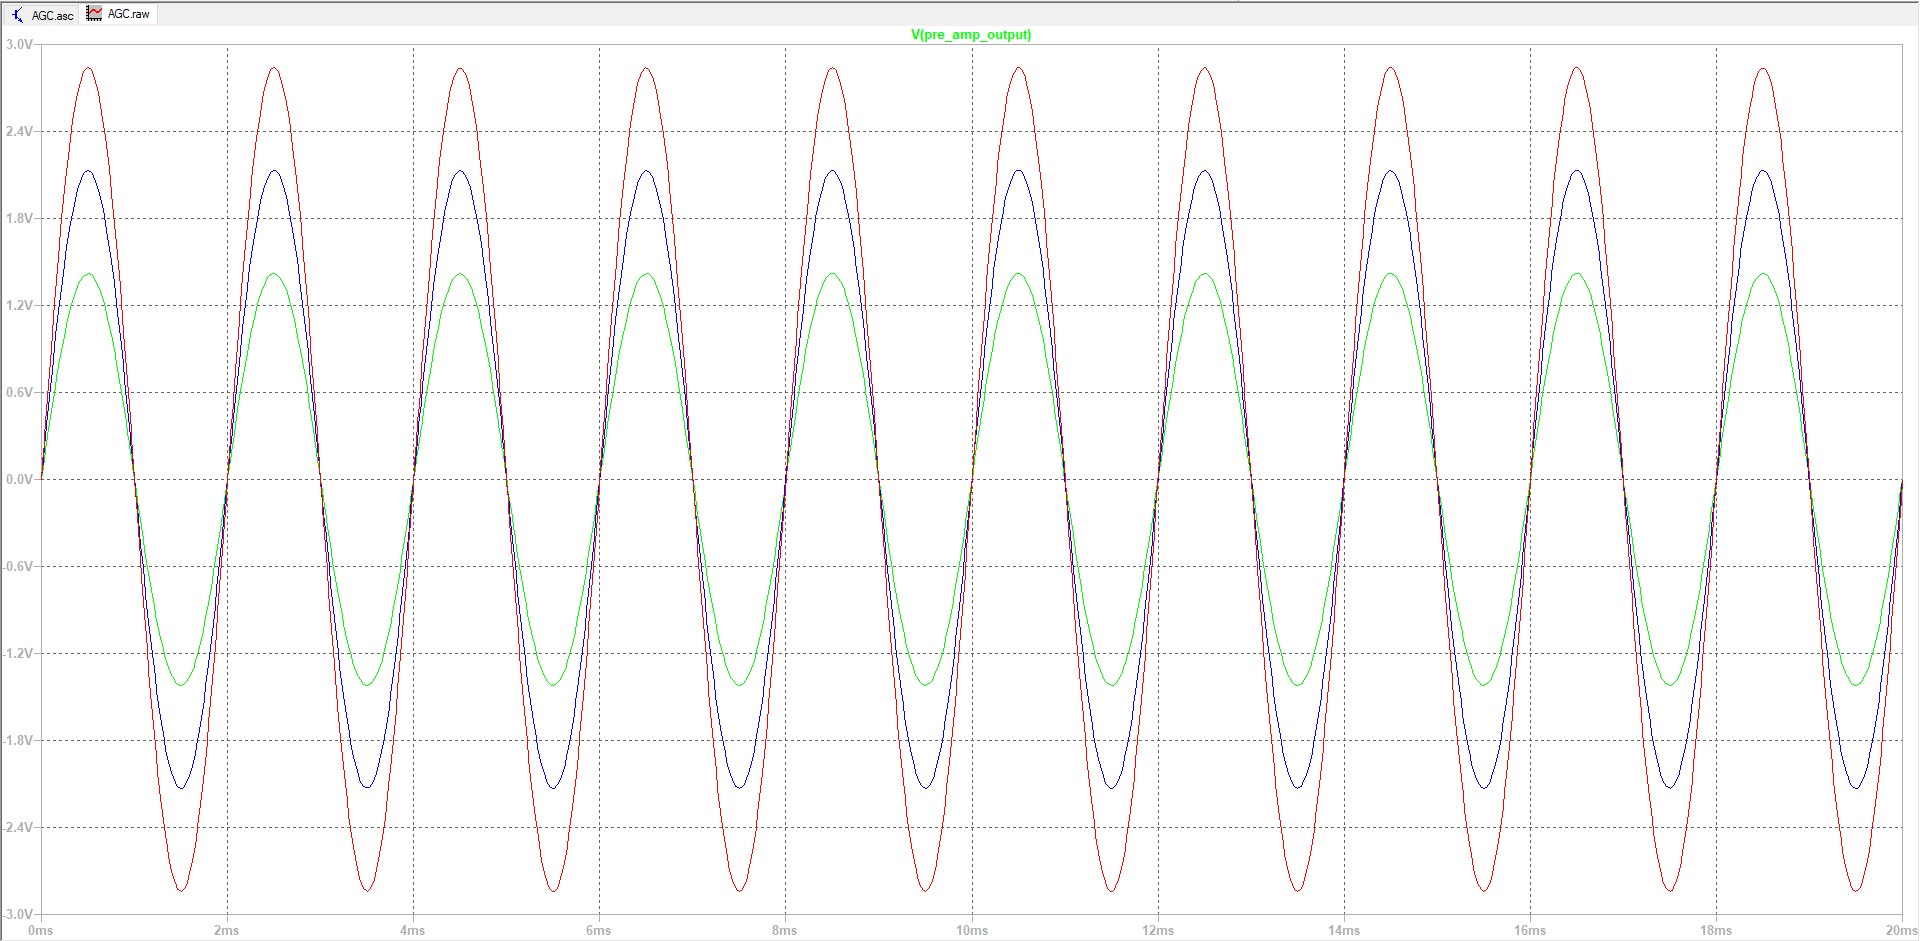
\includegraphics[width = 1\linewidth]{AGC Simulation Input.jpg}
    \caption{Automatic gain circuit simulation input.}
    \label{AGC_sim_input}
\end{figure} 
\begin{figure}[htbp!]
    \centering
    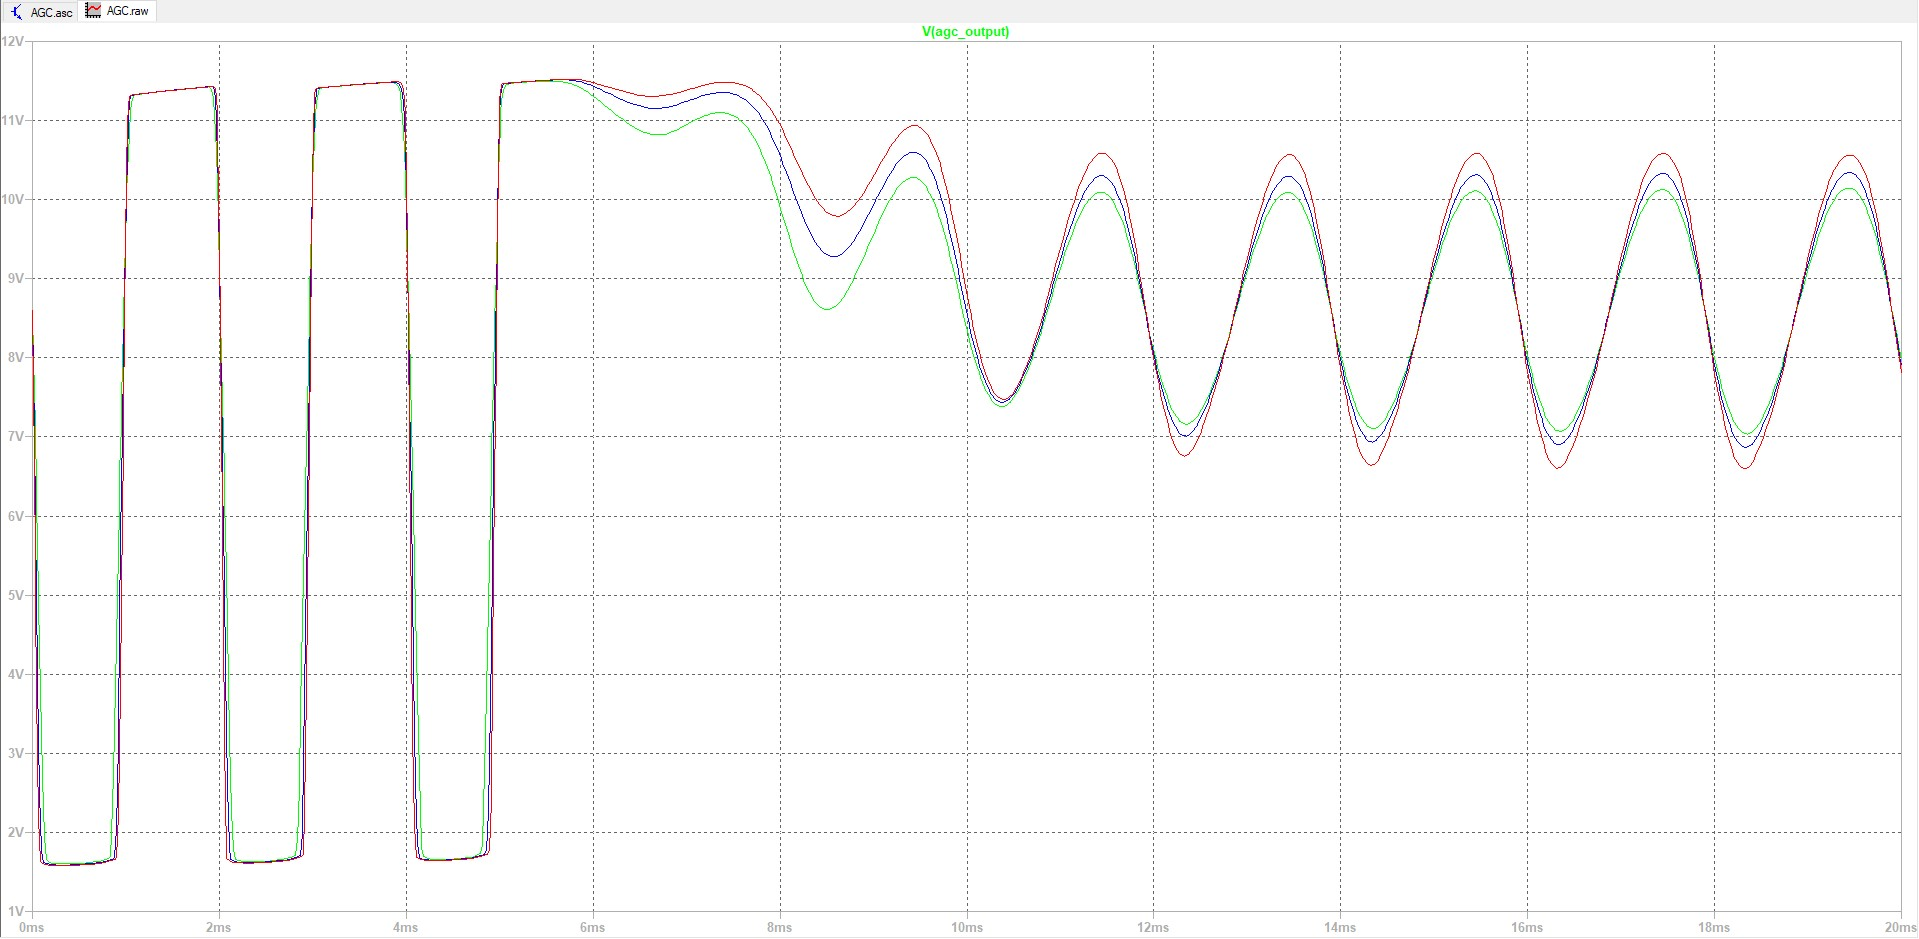
\includegraphics[width = 1\linewidth]{AGC Simulation Output.jpg}
    \caption{Automatic gain circuit simulation output.}
    \label{AGC_sim_output}
\end{figure} 
The experimental output of the AGC is given in Figure \ref{agc_osc}. The input is a 1khz sine wave sound played from a device.
\begin{figure}[htbp!]
    \centering
    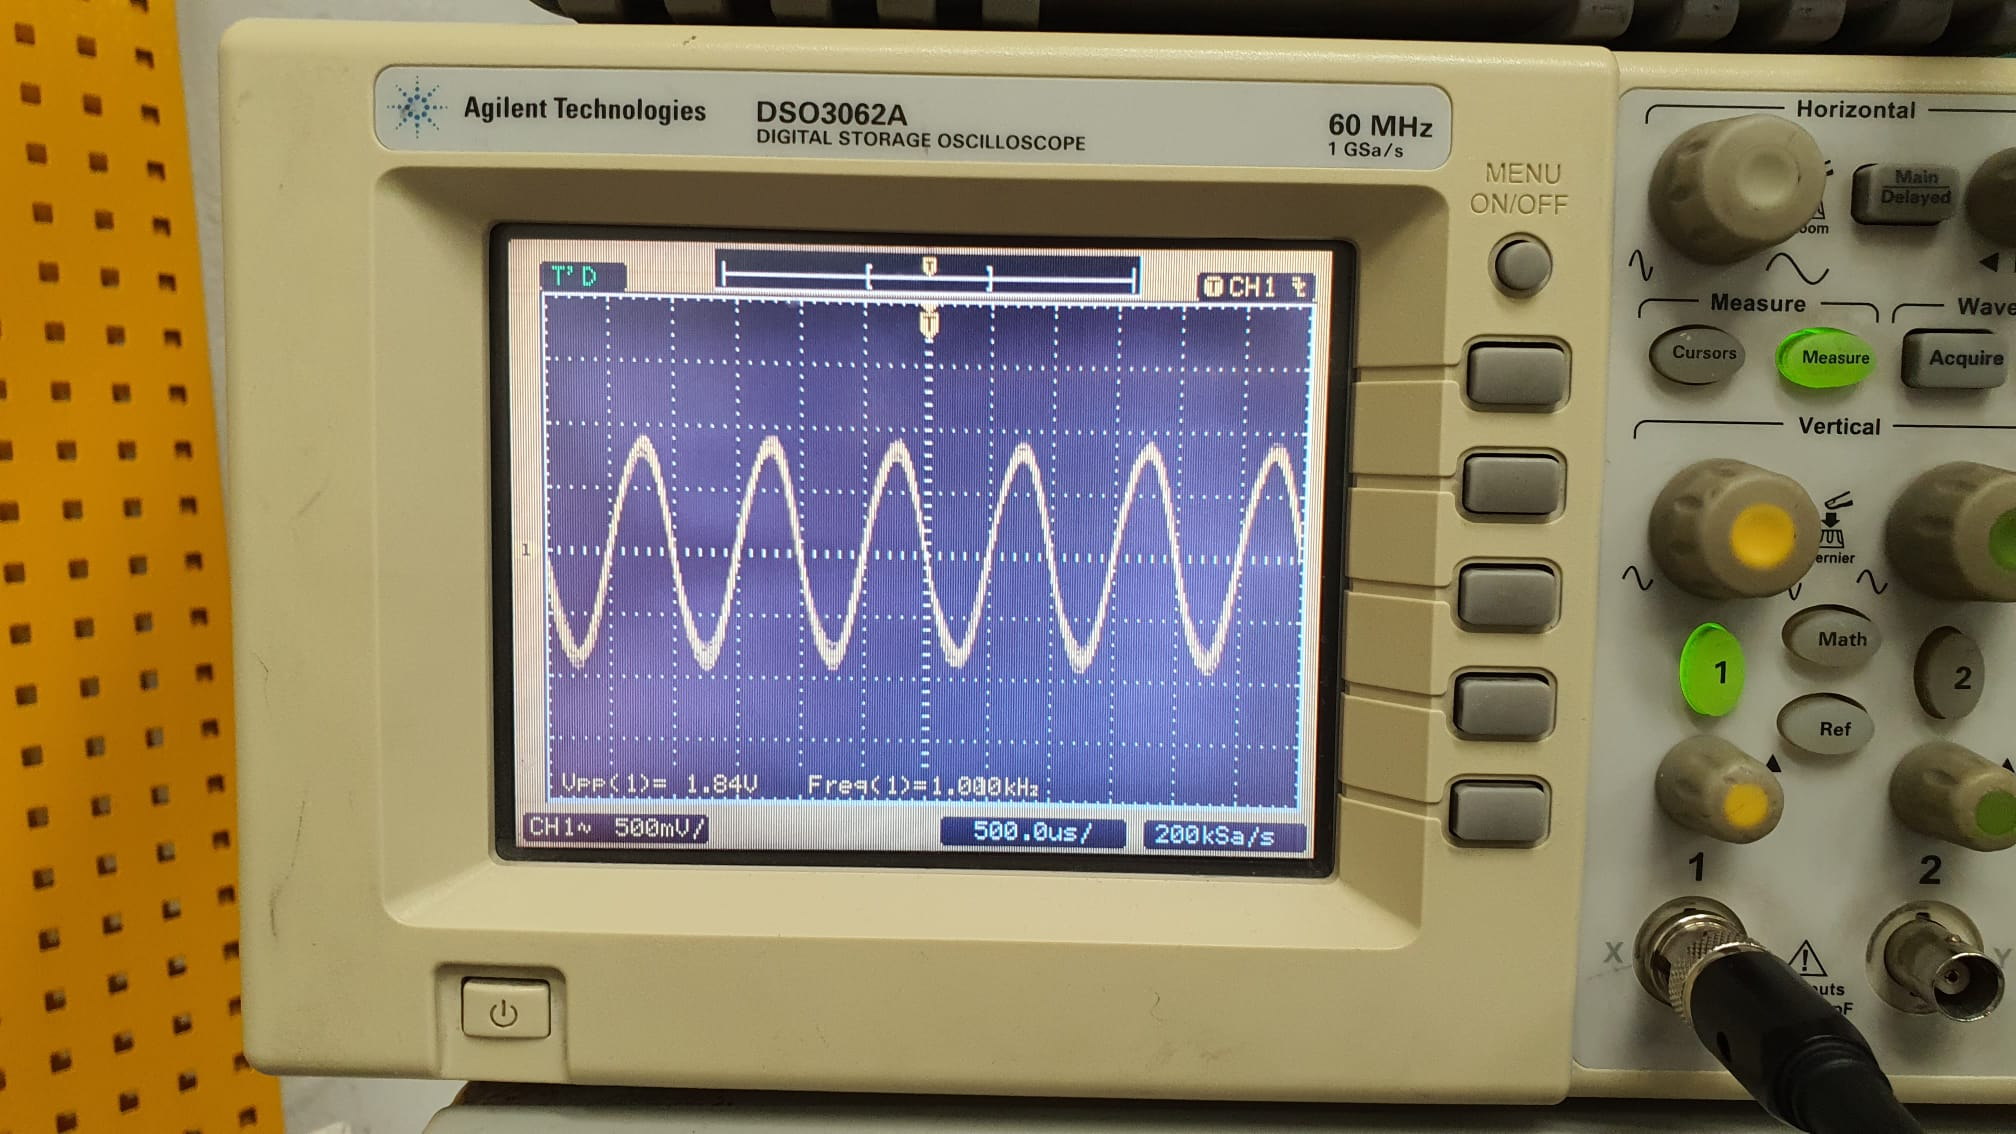
\includegraphics[width = 1\linewidth]{AGC_Experimental.jpeg}
    \caption{AGC circuit experimental result.}
    \label{agc_osc}
\end{figure} 
\subsection{Reference Signal Summation}

The constant gain audio signal and the high-frequency reference signal should be summed before transmission. This summation process is thought to be applied by adopting a simple op-amp summing amplifier.  The schematic is given in \ref{summing} is used in 1 to 1 ratio.
\begin{figure}[htbp!]
    \centering
    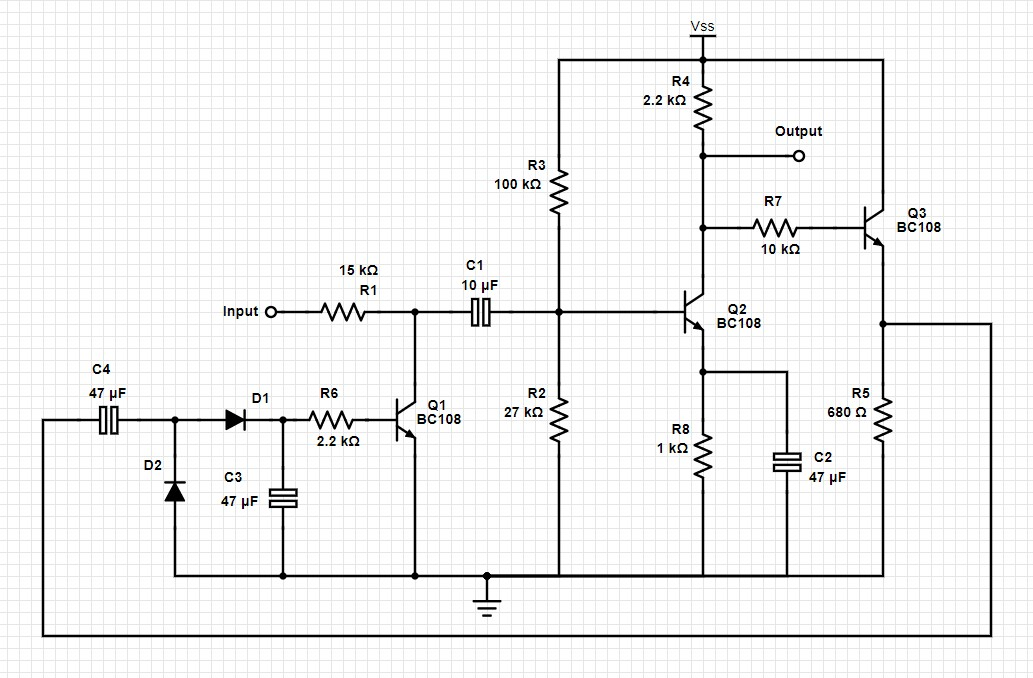
\includegraphics[width = 1\linewidth]{AGC Circuit.jpg}
    \caption{Summing amplifier.}
    \label{summing}
\end{figure} 
This circuit is a basic sum operator and 
\subsection{Light Transmission}
The decision on the light transmission is made towards using an IR LED. Since the LED's brightness changes with respect to the current pass thorugh it , we needed to convert the signal from voltage form to current form. In order achieve this we have utilized a transconductance amplifier given in Figure \ref{transconductance}. 
\begin{figure}[htbp!]
    \centering
    \includegraphics[width = 1\linewidth]{Led Driver Circuit.jpg}
    \caption{Transconductance amplifier.}
    \label{transconductance}
\end{figure} 
The circuit is composed of a basic degenerated common emitter configuration with a feedback. 

As a result of our prototyping process, we have constructed the circuit on a breadboard and the transmitter part of the circuit is successfully operated as expected without any big surprise. The physical structure of our prototype is given in Figure \ref{transmitter_breadboard} in Appendix.


\section{Receiver Side}
As shown in Figure \ref{general} the receiver design has two main branches after the light receiver. Therefore we have investigated them seperately.
\subsection{Light Receiver}
In the receiver section of the system, a photodiode is utilized to transform the optical signal into an electrical one. It's important to note that photodiodes are components that respond to current, so in order to convert the current into a voltage signal, a transresistance amplifier is employed. The design of the transresistance stage can be observed in Figure \ref{photodiode}. 
\begin{figure}[htbp!]
    \centering
    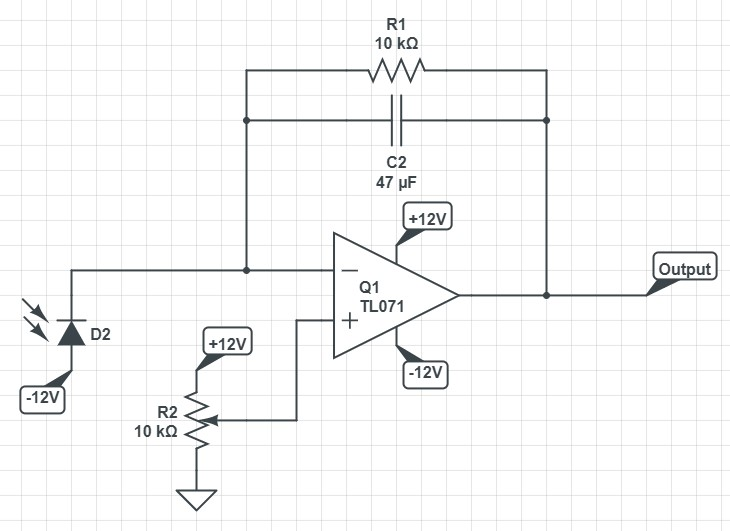
\includegraphics[width = 1\linewidth]{Photodiode amplifier.jpg}
    \caption{Photodiode amplifier. }
    \label{photodiode}
\end{figure} 
At the output of the light receiver an opamp buffer is emplyed for each input of a filter in order to maintain good signal quality on both inputs.
\subsection{Voice Signal Path}
\subsubsection{Low Pass Filter}
In order to extract the sound signal from inside of incoming signal a low-pass filter that is explained in the transmitter side is used. The circuit schematic is given in Figure \ref{lowpass} and the frequency response is given in Figure \ref{lowpass_resp}. We have constructed the given circuit and the experimental result is given in Figure \ref{lowpass_osc}.
\begin{figure}[htbp!]
    \centering
    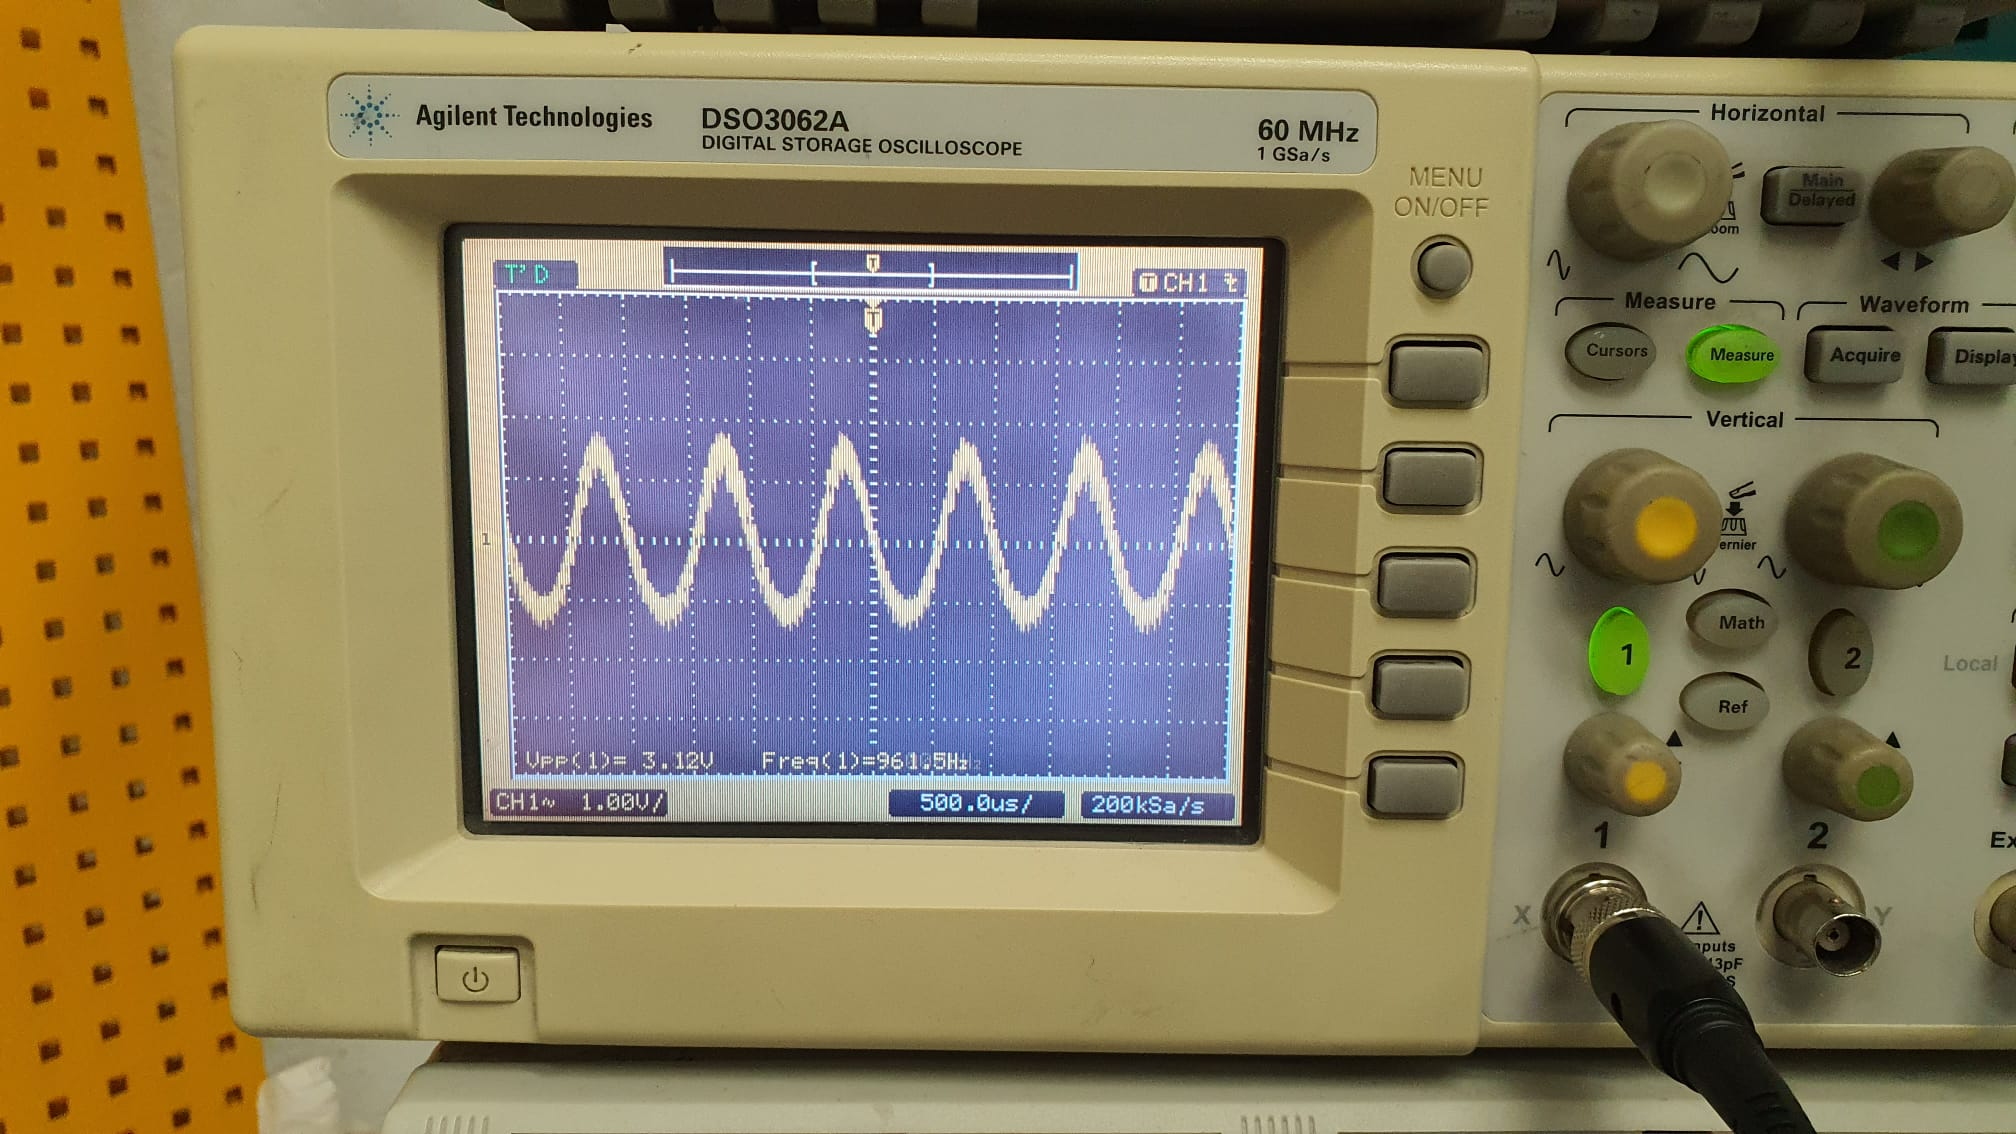
\includegraphics[width = 1\linewidth]{receiver_lowpass_experimental.jpeg}
    \caption{Experimental response of the lowpass filter at the receiver side. }
    \label{lowpass_osc}
\end{figure} 
Thus, it can be said that the intended use of the filter is achived.
\subsubsection{Speaker Driver}
After the process of filtering out high frequency signals, the original sound is obtained. This signal is then sent to the final stage for output, where power amplifiers with cooling components are utilized to power the speaker as op-amps alone are not capable of providing enough current. The specific type of output stage used in this scenario is known as a Class B output stage, which is more beneficial than Class A output stage since it offers relatively higher level of efficiency. A diagram of the speaker stage circuit can be found in Figure \ref{classb}.
\begin{figure}[htbp!]
    \centering
    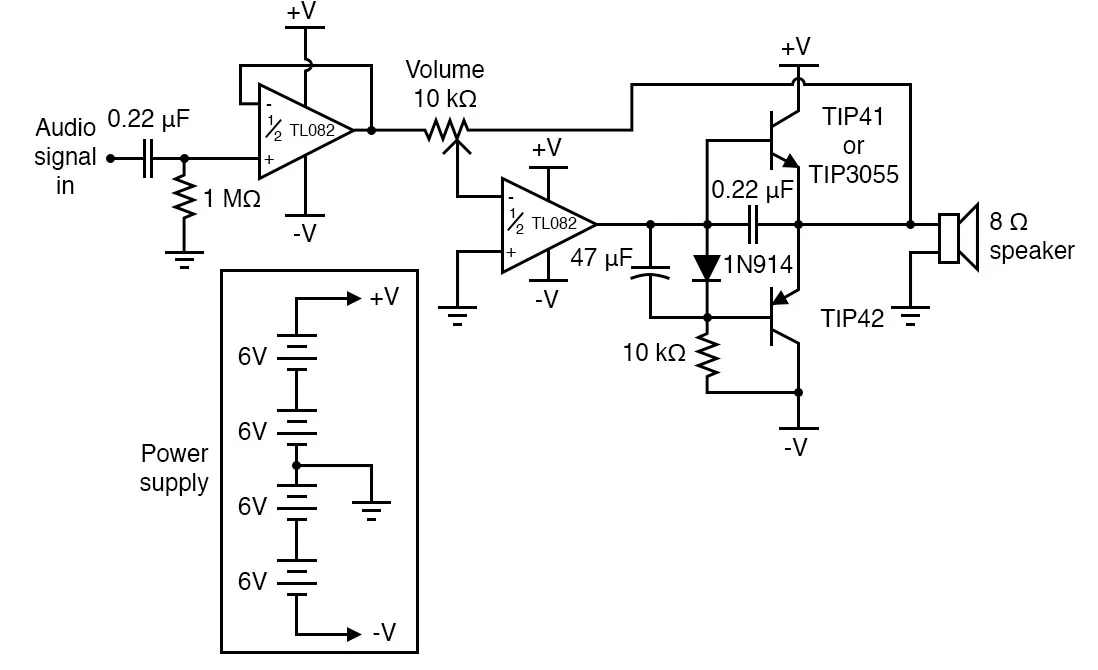
\includegraphics[width = 1\linewidth]{classb.png}
    \caption{Class B amplifier. }
    \label{classb}
\end{figure} 
The used topology also allows us to adjust the volume level easily without any compatibility or additional tuning for cascading two stages. The physical output of the amplifier is given in Figure \ref{speaker_osc}. That is the same 1kHz signal used in the first stage.
\begin{figure}[htbp!]
    \centering
    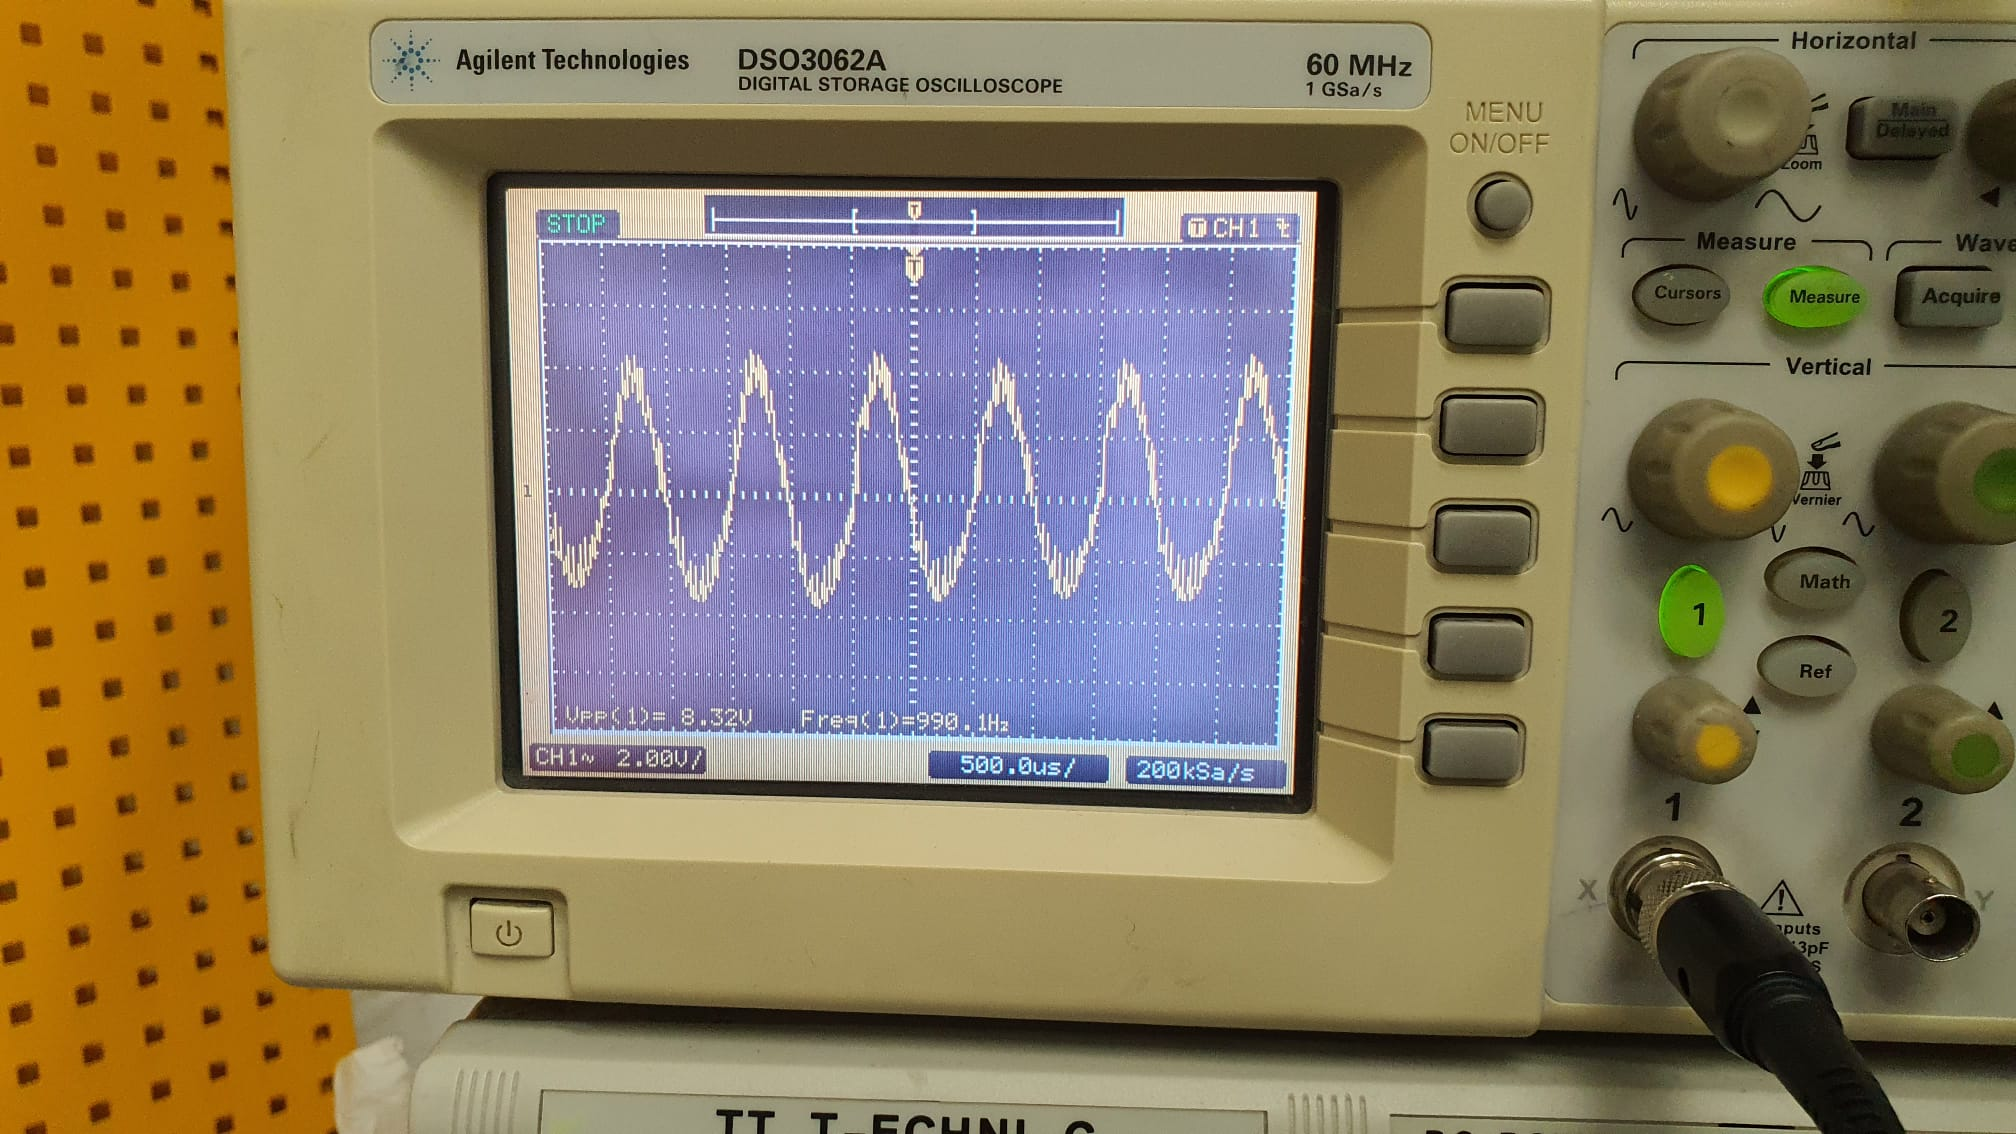
\includegraphics[width = 1\linewidth]{speaker_amplifier.jpeg}
    \caption{Experimental response of the speaker amplifier at the receiver side. }
    \label{speaker_osc}
\end{figure} 
\subsection{Carrier Signal Path}
\subsubsection{High Pass Filter}
To distinguish carrier signal from the  incoming overall signal. An active high-pass filter with sallen-key configuration  is used. The schematic is given in Figure \ref{highpass}.
\begin{figure}[htbp!]
    \centering
    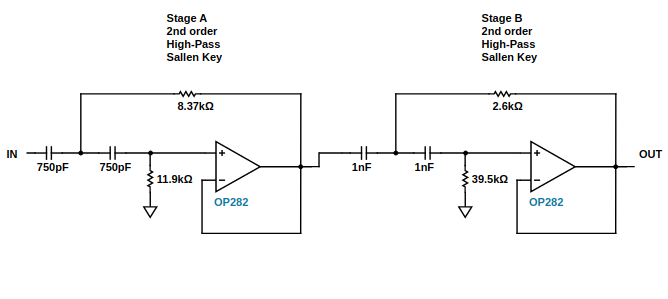
\includegraphics[width = 1\linewidth]{active_high_pass_circuit.png}
    \caption{High pass filter schematic. }
    \label{highpass}
\end{figure} 
The frequency response of the high-pass filter is given in Figure \ref{highpass_resp}.
\begin{figure}[htbp!]
    \centering
    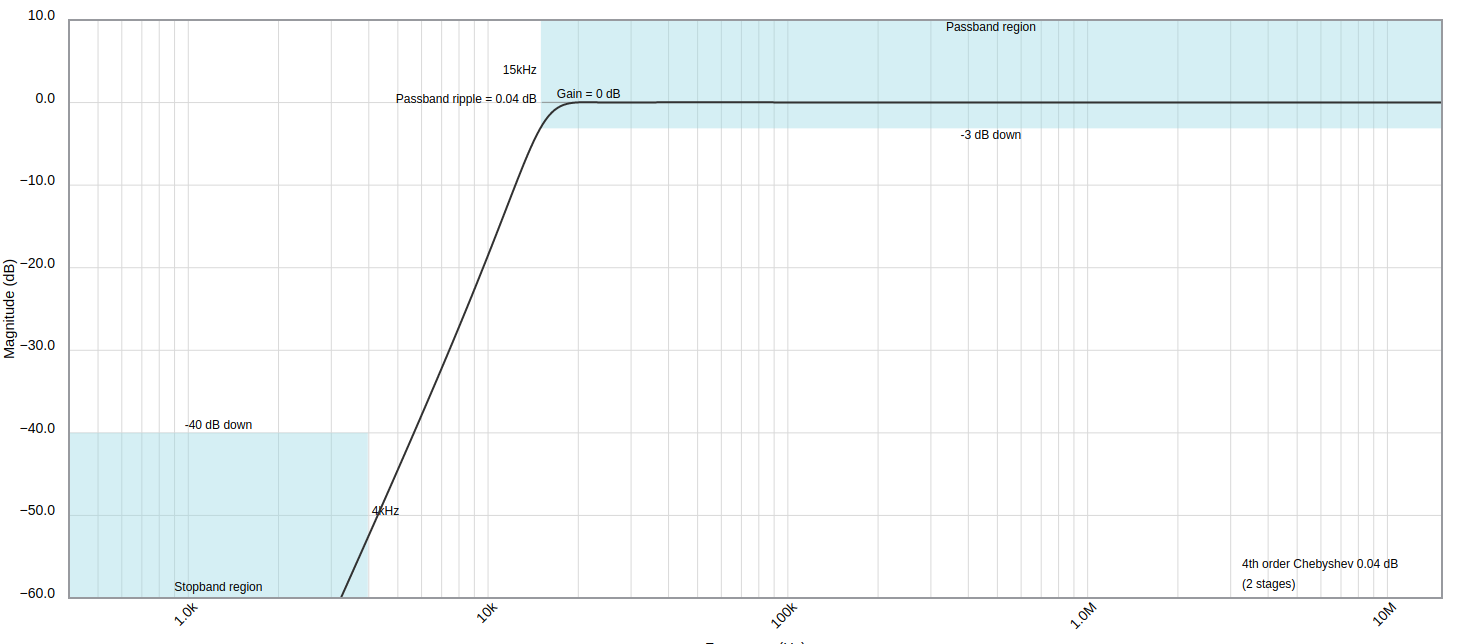
\includegraphics[width = 1\linewidth]{active_high_pass.png}
    \caption{High pass filter frequency response.}
    \label{highpass_resp}
\end{figure} 
\subsection{Peak Detector}
To be able to convert the sinusoidal signal coming from the high-pass filter to the DC logic levels. So we have utilized a two stage peak detector which has almost no ripple compared the its DC average. The circuit schematic is given in Figure \ref{peak}.
\begin{figure}[htbp!]
    \centering
    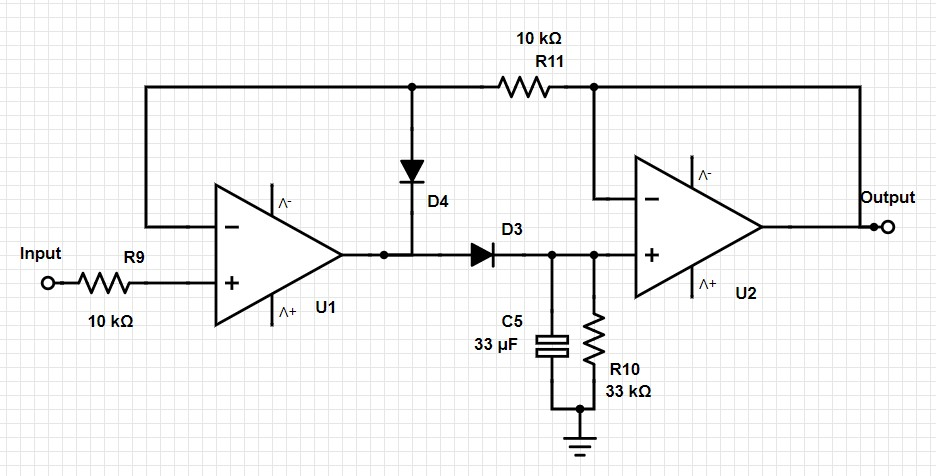
\includegraphics[width = 1\linewidth]{Peak Detector.jpg}
    \caption{Peak detector circuitry.}
    \label{peak}
\end{figure} 
\subsubsection{Signal Level Indication}
At the last stage of the carrier signal pathway, the a comparator array composed of op-amps drives an RGB LED to indicate the level of the incoming signal. Figure \ref{array} shows how the configuration works.
\begin{figure}[htbp!]
    \centering
    \includegraphics[width = 1\linewidth]{Led Driver Circuit.jpg}
    \caption{Comparator array.}
    \label{array}
\end{figure}
The scheme of how the signal levels corresponds to the colors are given in Table \ref{tab:array}


\begin{table}[]
    \caption{the color scheme}
    \label{tab:array}
    \begin{tabular}{|cc|cc|cc|cc|}
    \hline
    \multicolumn{2}{|c|}{\textbf{Reference 1}}          & \multicolumn{2}{c|}{\textbf{Reference 2}}            & \multicolumn{2}{c|}{\textbf{Reference 3}}            & \multicolumn{2}{c|}{\textbf{Reference 4}}            \\ \hline
    \multicolumn{1}{|c|}{\textit{red}} & \textit{red}   & \multicolumn{1}{c|}{\textit{red}}   & \textit{}      & \multicolumn{1}{c|}{\textit{}}      & \textit{}      & \multicolumn{1}{c|}{\textit{}}      & \textit{red}   \\ \hline
    \multicolumn{1}{|c|}{\textit{}}    & \textit{green} & \multicolumn{1}{c|}{\textit{green}} & \textit{green} & \multicolumn{1}{c|}{\textit{green}} & \textit{green} & \multicolumn{1}{c|}{\textit{green}} & \textit{green} \\ \hline
    \multicolumn{1}{|c|}{\textit{}}    & \textit{}      & \multicolumn{1}{c|}{\textit{}}      & \textit{}      & \multicolumn{1}{c|}{\textit{}}      & \textit{blue}  & \multicolumn{1}{c|}{\textit{blue}}  & \textit{blue}  \\ \hline
    \end{tabular}
\end{table}
    
\section{Conclusion}
In this project, we delved deeper into the intricacies of analog circuit design by applying the theoretical concepts learned in our EE311 and EE313 courses. Our focus was on optical wireless communication systems, and through our study of these systems, we gained a comprehensive understanding of their principles of operation. We explored new circuit designs such as transconductance and transresistance amplifiers, and learned how they can be applied in practical settings. Additionally, we gained valuable hands-on experience in implementing peak detector and speaker driver circuits. As we encountered and overcame any difficulties that arose during the course of the project, we developed a greater appreciation for the complexities and nuances of analog circuit design. Through this project, we were able to enhance our understanding of the fundamental concepts and principles that govern the functioning of analog circuits and gained a deeper understanding of their real-world applications.
\section*{Appendix}
The physical model of our system is presented in Appendix.
\begin{figure}[htbp!]
    \centering
    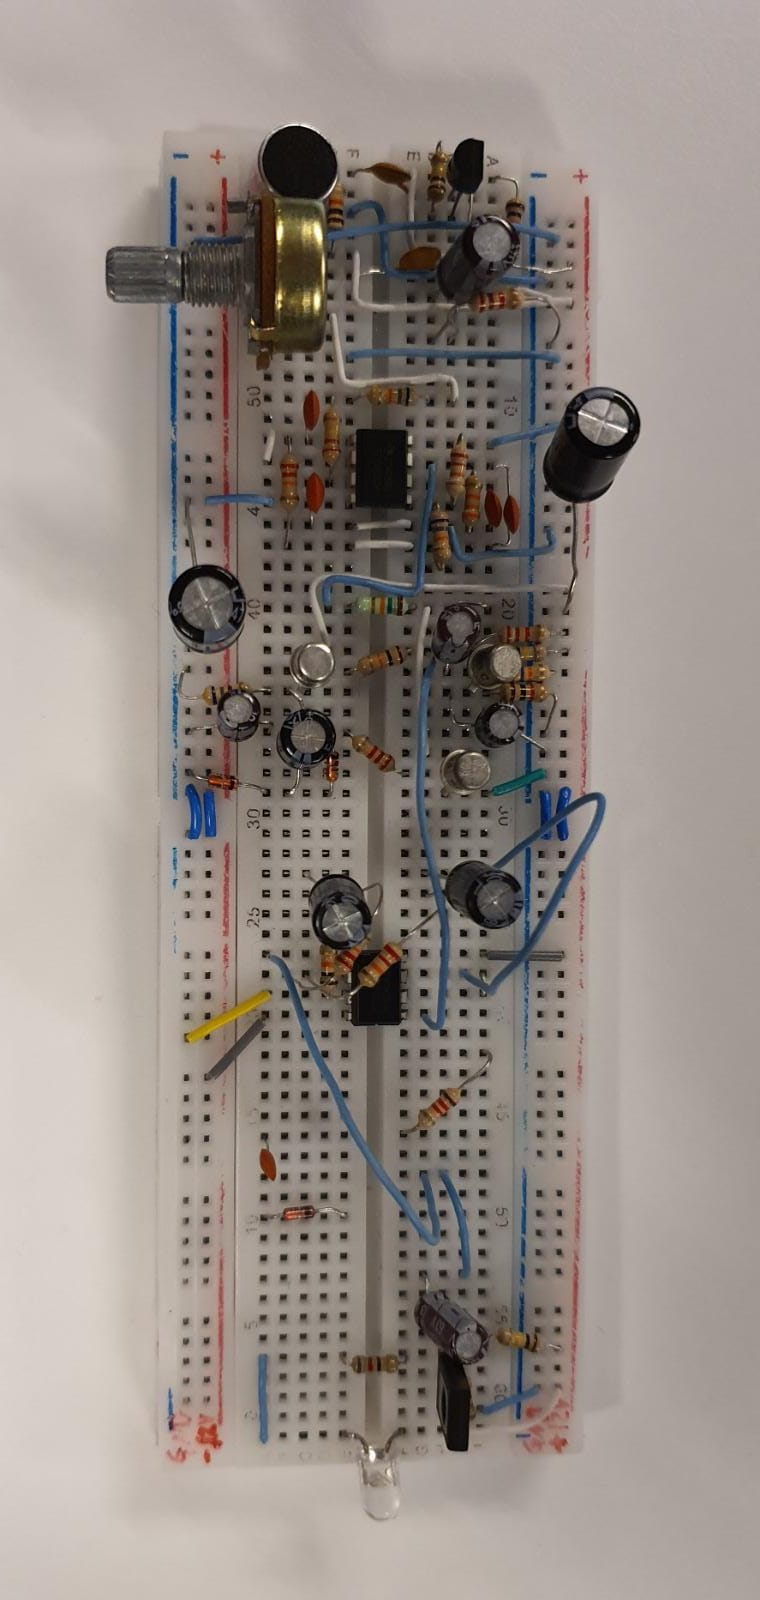
\includegraphics[width = 1\linewidth]{transmitter.jpeg}
    \caption{Transmitter prototype.}
    \label{transmitter_breadboard}
\end{figure} 
\end{document}

%%%%%%%%%%%%%%%%%%%%%%   EXAMPLE TABLE   %%%%%%%%%%%%%%%%%%%%%%%%%%%%%%%%
\begin{table}[H]
\begin{center}
    \caption{Resistance reading by color code convention.}
    \vspace{2mm}
    \begin{tabular}{||c | c | c||} 
        \hline
        Color Order & Value & Tolerance \\ [0.5ex] 
        \hline\hline
        Brown / Black / Red / Gold & 1k\( \Omega \) & \( \% \) 5  \\ 
        \hline
        Yellow / Violet / Red / Gold & 4.7k\( \Omega \) & \( \% \) 5   \\
        \hline
        Brown / Grey / Orange / Gold & 18k\( \Omega \) & \( \% \) 5  \\ [1ex] 
        \hline
    \end{tabular}
\end{center}
\end{table}


%%%%%%%%%%%%%%%%%%%%%%   EXAMPLE IMAGE   %%%%%%%%%%%%%%%%%%%%%%%%%%%%%%%%
\begin{figure}[H]
\centering
\includegraphics[width = 0.75\linewidth]{5.png}
\caption{Circuit schematic for the step 5}
\end{figure} 

%%%%%%%%%%%%%%%%%%%%%%   EXAMPLE IMAGE FROM PDF   %%%%%%%%%%%%%%%%%%%%%%%%%%%%%%%%
\begin{figure}[H] \centering{
    \includegraphics[scale=0.25]{2a_plot.pdf}}
    \caption{Experiment 2}
\end{figure}
%%%%%%%%%%%%%%%% Deneme Push